\documentclass[xcolor=x11names,table]{beamer}

%HOUT \documentclass[handout,english,basque]{beamer}
%Cambios de color
\include{tikzSetup}
%Paleta
\usepackage{xcolor}

\definecolor{azulfct}{RGB}{0,42,96}
\definecolor{gris}{RGB}{90,95,97}
\definecolor{azul}{RGB}{0,112,255}
\definecolor{naranja}{RGB}{255,143,0}
\definecolor{blanco}{RGB}{255,255,255}

\definecolor{myblue}{rgb}{0.086, 0.3098, 0.5255} % 154F86
\definecolor{mybluedd}{HTML}{2b8cbe} %Dark HTML
\definecolor{myblueddd}{HTML}{173753} %Dark HTML 173753
\definecolor{mybluedddd}{HTML}{1B4353} %DarkDark HTML 1B4353
\definecolor{myblueF}{HTML}{23516d} % 154F86
\definecolor{myblue5}{rgb}{0.08,0.58,0.89}
\definecolor{mybluel}{HTML}{3E75a9} %Light  6DAEDB
\definecolor{mybluell}{HTML}{2d5d8a} %LightLight


%del fichero beamercolorthemebeaver.sty
\setbeamercolor{structure}{fg=azulfct}
% \setbeamercolor{structure}{fg=azul} %Cambiado

\setbeamercolor{palette primary}{fg=azulfct,bg=gris!70}
\setbeamercolor{palette secondary}{fg=azulfct,bg=gris!80}
\setbeamercolor{palette tertiary}{fg=azulfct,bg=gris!90}
\setbeamercolor{palette quaternary}{fg=azulfct,bg=gris}

% \setbeamercolor{titlelike}{parent=palette quaternary}
% 
% \setbeamercolor{block title}{fg=azulfct,bg=gris}
% \setbeamercolor{block title alerted}{use=alerted text,fg=azulfct,bg=alerted text.fg!75!bg}
% \setbeamercolor{block title example}{use=example text,fg=azulfct,bg=example text.fg!75!bg}
% 
% \setbeamercolor{block body}{parent=normal text,use=block title,bg=block title.bg!25!bg}
% \setbeamercolor{block body alerted}{parent=normal text,use=block title alerted,bg=block title alerted.bg!25!bg}
% \setbeamercolor{block body example}{parent=normal text,use=block title example,bg=block title example.bg!25!bg}
% 
% \setbeamercolor{sidebar}{bg=gris!70}
% 
% \setbeamercolor{palette sidebar primary}{fg=azulfct}
% \setbeamercolor{palette sidebar secondary}{fg=azulfct!75}
% \setbeamercolor{palette sidebar tertiary}{fg=azulfct!75}
% \setbeamercolor{palette sidebar quaternary}{fg=azulfct}

% \setbeamercolor*{separation line}{}
% \setbeamercolor*{fine separation line}{}


%%Mis cambios

\setbeamercolor{frametitle}{fg=azulfct,bg=gris}
\setbeamercolor{normal text}{fg=azulfct}


% \usepackage[utf8]{inputenc}  %parece que no hace falta con xelatex
% \usepackage{default}

%La plantilla
% \usetheme{Goettingen}

%Para que los itemize sean circulos
\useinnertheme{circles}


\usepackage[no-math]{fontspec}
\setsansfont{EHUSans}
%Para algún texto particular
\newfontfamily\myEHUSerif{EHUSerif}     %Uso, entre paréntesis si es necesario   \my_EHUSerif
 


% \usepackage[many]{tcolorbox}
% \makeatletter
% \setbeamertemplate{frametitle}{%
%   \nointerlineskip%
%   \usebeamerfont{headline}%
%   \nointerlineskip%
%   \hbox{\hspace{-0.09\paperwidth}%
%   \begin{tcolorbox}[
%     enhanced,
%     boxrule=0pt,   %Elimino un caja de 15pt que ponía a la izquierda
%     colframe=naranja,
%     arc=0pt,
%     outer arc=0pt,
%     colback=green,
%     colupper=naranja,
%     width=\paperwidth+2mm,
%     toprule=0pt,
%     bottomrule=0pt,
%     rightrule=0pt,
%     left=15pt,
%   ]%
% %    {\usebeamercolor{frametitle}\usebeamerfont*{frametitle}\strut\insertframetitle\strut} Quito dos strut que meten un espacio y hacen el frametitle más ancho
%     {\usebeamercolor{frametitle}\usebeamerfont*{frametitle}\insertframetitle}
%     \ifx\insertframesubtitle\@empty%
%       \strut\par%
%     \else%
%      \par{\usebeamerfont*{framesubtitle}{\usebeamercolor[fg]{framesubtitle}\insertframesubtitle}\par}%
%     \fi
%   \end{tcolorbox}%
%   }
%   \hrule width \paperwidth heigh 100pt
% 
%   \nointerlineskip
% }
% \makeatother


\setbeamertemplate{frametitle}{%
    \usebeamerfont{frametitle}\vspace{.2\baselineskip}\insertframetitle%
    \vphantom{g}% To avoid fluctuations per frame
    %\hrule% Uncomment to see desired effect, without a full-width hrule
    \par% <-- added
    
    \ifx\insertframesubtitle\@empty%
      \strut\par%
    \else%
     \par{\usebeamerfont*{framesubtitle}{\usebeamercolor[fg]{framesubtitle}\vspace{.3\baselineskip}\insertframesubtitle}\par}%
    \fi     
    \hspace*{-\dimexpr0.5\paperwidth-0.5\textwidth}% <-- calculation of left margin width
    %a paperwidth=128mm=364.16pt   1mm=2.845pt 
%Para 4/3    
%     \mbox{\rule[.4\baselineskip]{224.59pt}{1pt}\hspace{1pt}%  % para que sea una continuación de linea, sino introduce `` ''
% \rule[.4\baselineskip]{85.17pt}{1pt}\hspace{1pt}%
% \rule[.4\baselineskip]{31.91pt}{1pt}\hspace{1pt}%
% \rule[.4\baselineskip]{11.57pt}{1pt}\hspace{1pt}%
% \rule[.4\baselineskip]{3.80pt}{1pt}\hspace{1pt}%
% \rule[.4\baselineskip]{1pt}{1pt}
%Para 16/9    
    \mbox{\rule[.4\baselineskip]{279.82pt}{1pt}\hspace{1pt}%  % para que sea una continuación de linea, sino introduce `` ''
\rule[.4\baselineskip]{105.46pt}{1pt}\hspace{1pt}%
\rule[.4\baselineskip]{40.05pt}{1pt}\hspace{1pt}%
\rule[.4\baselineskip]{14.68pt}{1pt}\hspace{1pt}%
\rule[.4\baselineskip]{5.99pt}{1pt}\hspace{1pt}%
\rule[.4\baselineskip]{2.29pt}{1pt}\hspace{1pt}%
\rule[.4\baselineskip]{1pt}{1pt}
}
\vspace{-.5em}  % subo un poco porqu si no el texto principal empiza muy abajo
}



%Para las imagenes
\usepackage{graphicx}
\graphicspath{{Images/}}
%Para fijar imagenes
\usepackage[absolute,overlay]{textpos}   % añadir ,showboxes para ver la caja de texto, no tiene borde por abajo, es donde empieza el texto y de ahí para abajo
\setlength{\TPHorizModule}{128mm}   % 1 unidad de ancho es textpos es el ancho de la diapositiva
\setlength{\TPVertModule}{96mm}     % 1 unidad de alto es textpos es el ancho de la diapositiva


%Kentzen ditugu beheko nabigatzeko botoiak
\setbeamertemplate{navigation symbols}{}

%Page number esto pone 10/96
% \setbeamertemplate{footline}[frame number]
% Esto quita el numero total de frames
\setbeamertemplate{footline}{% 
  \hfill% 
  \usebeamercolor[fg]{page number in head/foot}% 
  \usebeamerfont{page number in head/foot}% 
  \insertframenumber%
  %\,/\,\inserttotalframenumber
  \kern1em\vskip2pt% 
}


%Multirow
\usepackage{multirow}


%Para las citas de la esquina
% \usepackage[absolute]{textpos}
% \setlength{\TPHorizModule}{10mm}
% \setlength{\TPVertModule}{\TPHorizModule}
\usepackage{tikz}
\usepackage[]{media9}


%%% Time in presentation

\usepackage[font=Times,timeinterval=1, timeduration=2.0, timedeath=0, fillcolorwarningsecond=white!60!yellow,
timewarningfirst=50,timewarningsecond=80,resetatpages=all]{tdclock}

\usepackage{cancel}
\usepackage{amsmath}
\usepackage{listings}
\usepackage{animate}
\usepackage{setspace}
\usepackage{changepage}
\usepackage{caption}
\usepackage{textpos}
\usepackage{fancybox}
\usepackage{pstricks}
\usepackage{media9}
\usepackage{tabu}
\hypersetup{pdfpagemode=UseNone}

\usepackage{colortbl}
\usepackage{overpic}
\usepackage{geometry}
\usepackage{pdfpcnotes}

\usepackage[basque]{babel}

\newcommand{\specialcell}[2][l]{%
 \begin{tabular}[#1]{@{}l@{}}#2\end{tabular}}

\usepackage{caption}
\usepackage{eurosym}

\usepackage{listings}

\makeatletter%
\special{pdf: put @thispage <</Group << /S /Transparency /I true /CS /DeviceRGB>> >>}%
\makeatother%

\makeatletter
\let\@@magyar@captionfix\relax
\makeatother

\usepackage{ragged2e}



%HOUT \input{hout}
%HOUT \addtobeamertemplate{frametitle}{\vspace*{-1.4cm}}{\vspace*{0.2cm}}

\usepackage{amsmath, amssymb, graphics, setspace}
\usepackage[utf8x]{inputenc}
%\usepackage[english]{babel}
%\usepackage{url}
%\newcommand{\mathsym}[1]{{}}
%\newcommand{\unicode}[1]{{}}

%\newcounter{mathematicapage}
\usepackage{listings}
% for placeholder text
\usepackage[framemethod=TikZ]{mdframed}

%%%%%%
% Taken from https://tex.stackexchange.com/questions/84748/fanciest-way-to-include-mathematica-code-in-latex
\usepackage{lmodern}

%\usepackage{mmacells}


%%%%%



\title{{\tt Mathematica} eta Mekanika Kuantikoa.  }
\author{Ion Mitxelena, Davide de Sancho, Txema Merecero \\ eta \\ Xabier Lopez}

\begin{document}
\maketitle


\section{{\tt Mathematica.} Oinarrizko kontzeptuak }
\begin{frame}{Aurkibidea}

\tableofcontents{}
\end{frame}
\begin{frame}{\tt Mathematica}
	
{\tt Mathematica}-n maiuskula eta minuskulak bereizten dira, eta parentesi mota 
desberdinek esanahi desberdina dute:

\begin{itemize}
	\item<2-> {[ ]} funtzioen aldagaiak adirezteko erabiltzen dira. {\tt Sin[x]}.
			 
	\item<3-> () Eragiketak taldekatzeko erabiltzen da. {\tt (6+4)/2}.
	\item<4-> \{\} zerrendak edo segidak definitzeko erabilzten dira. {\tt \{X,0,10,1\}}.
%	\item (* *) parentesi tartean dagoena komentario bat dela adierazten du.
	\item<5-> Ohiko ariketa matematikoak egiten ditu ohiko ikurrekin: { +, -, /, \textasciicircum , Sqrt }...
	\item<6-> Hainbat funtzio ere baditu definituta: {\tt Sin, Cos, Log }... 
		guztiak hizki maiuskula batekin hasiko direlarik. 
	\item<7-> Definitutako aldagaika ere inprima daitazke Print aginduarekin.
\end{itemize}

\onslide<8->{Definizio, edo eragiketa baten emaitza ikusteko, {\tt SHIFT+ENTER} sakatu behar da. 
Bestalde, definizio baten atzekaldean {\tt ;} adierazten bada, definizio horren 
emaitza ez da erakutsiko. Ez bada jartzen ordea, 
definizioaren emaitza idatziko du {\tt Mathematica}-k.}
\end{frame}

\begin{frame}[fragile]
\begin{mdframed}[backgroundcolor=gray!05,roundcorner=2pt]
	\begin{itemize}
		\item<1-> f=2(* f-k bi balio du *)

		\item<2-> 2
		\item<3-> j=5;
		\item<3-> h=f*j

		\item<4-> 10

		\item<5-> 5$\textasciicircum$3

		\item<6-> 125

		\item<7-> Print[f]
		\item<8-> 2


		\item<9-> har=627.5;(* hartree bat 627.5 kcal/mol *)
		\item<9-> En=0.023;
		\item<9-> $ Print[En, " hartree ", En*har, " kcal/mol\quad dira "] $

		\item<10-> 0.023 hartree 14.4325 kcal/mol dira
	\end{itemize}
\end{mdframed}
\end{frame}
%\end{document}

%%%%%%%%%%%%%%%%%



%Aldagai bati balio zehatz bat eslitzeko {\tt =} keinua erabiliko da, bestalde funtzio
%bat defintzeko garaian {\tt := } erabiliko dugu, non berdintasuna ez da zuzenean 
%interpretatzen.

\begin{frame}{Funtzioak definitzen}

\begin{mdframed}[backgroundcolor=gray!05,roundcorner=2pt]

	\begin{itemize}
		\item<1-> x=2;
		\item<1->  fa=4+x;
		\item<1->  fb:=4+x;
		\item<1-> Print[fa]


		\item<2-> 6


		\item<3-> Print[fb]


		\item<4->  6


		\item<5-> T{x}=4;
		\item<5-> Print[fa]

		\item<6-> 6

			\item<7-> Print[fb]


		\item<8-> 8
	\end{itemize}
\end{mdframed}
\end{frame}


\begin{frame}{Funtzioak irudikatzen}

	\begin{itemize}
		\item<2-> a=1; b=1; c=1 ;
		\item<1-> Plot[a*x$\textasciicircum$4+b*x$\textasciicircum$2+c*x+2,\{x,-20,20\}] 
	\end{itemize}

	\begin{center}
		\onslide<3->{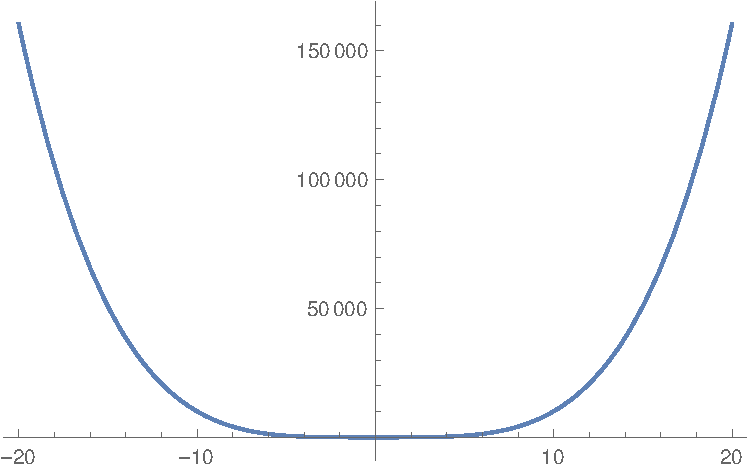
\includegraphics[scale=0.5]{f1.pdf}}
	\end{center}
\end{frame}

\begin{frame}{Funtzioak irudikatzen}
\begin{itemize}
		\item<1-> Manipulate[Plot [a*x$\textasciicircum$4+b*x$\textasciicircum$2+c*x+2,\{x,-20,20\}, \\
 PlotRange -> \{\{-20, 20\}, \{-20, 20\}\}],\\
 \{a, -1, 1\}, \{b, -10, 10\}, \{c, -10, 10\} ] 
\end{itemize}
\vspace{-1.5cm}
\begin{center}
\onslide<2->{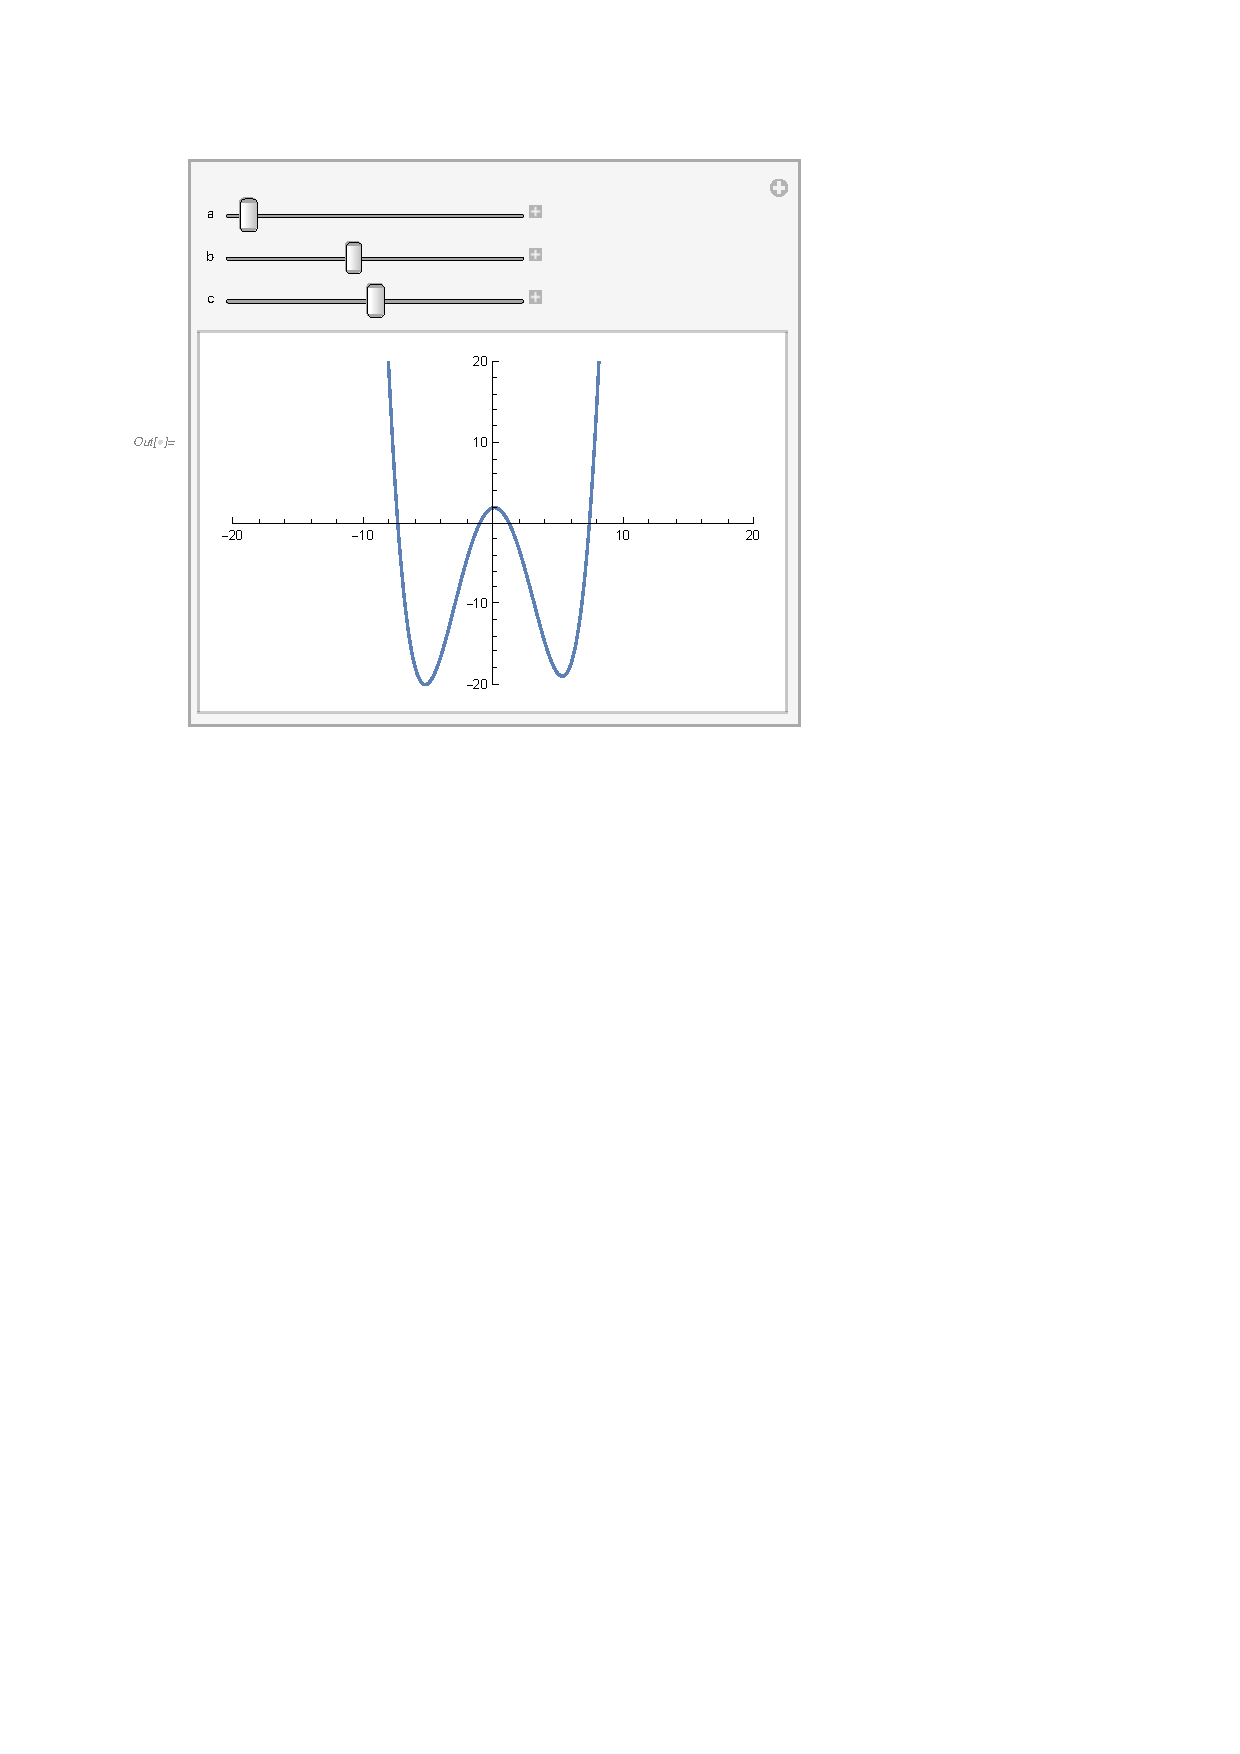
\includegraphics[scale=0.6]{f0.pdf}}
\end{center}

\end{frame}
%%%%%%%%%%
\begin{frame}{Funtzioak irudikatzen}
\begin{itemize}

\item<1->  sph[x\_, y\_, z\_] := x$\textasciicircum$2 + y$\textasciicircum$2 + z$\textasciicircum$2;\\ 
           ContourPlot3D[sph[x, y, z] == 1, \{x, -1, 1\}, \{y, -1, 1\}, \{z, -1, 1\}]

\end{itemize}
\begin{center}
\onslide<2->{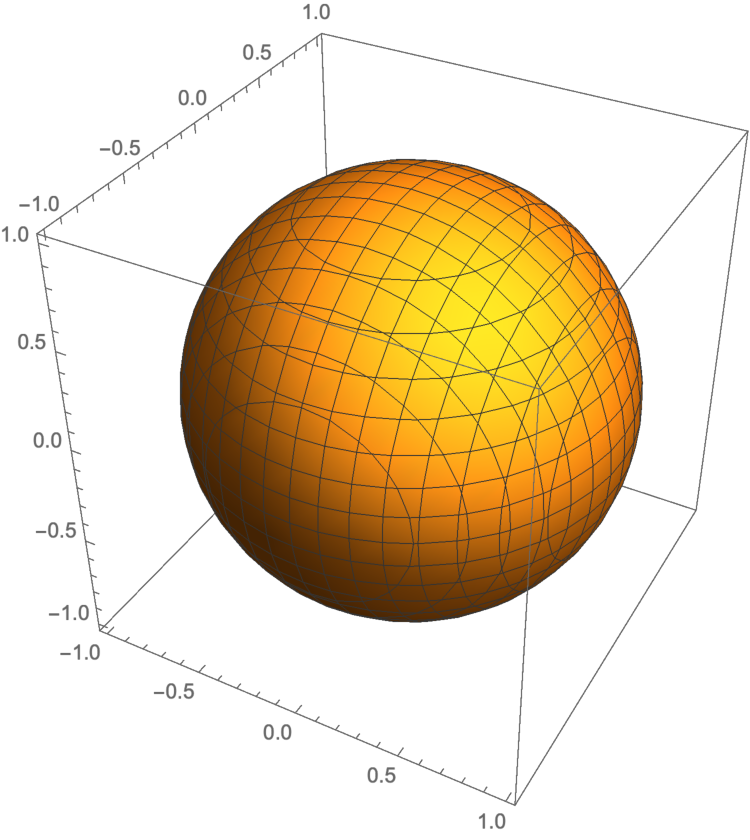
\includegraphics[scale=0.5]{f2.pdf}}
\end{center}
\end{frame}

\begin{frame}{Deribatuak}
\begin{itemize}
	\item <1-> f[x\_] := 3 $\textasciicircum$2 + 7;
	\item <1-> f \ '[x]
	\item <2-> 6x
		\item <3-> f[x\_] := (Sin[x])$\textasciicircum$2; 
		\item <3-> Plot[\{f'[x], Sin[x], Cos[x]\},\{x, 0, 2 Pi\}]
\end{itemize}
\begin{center}
\onslide<4->{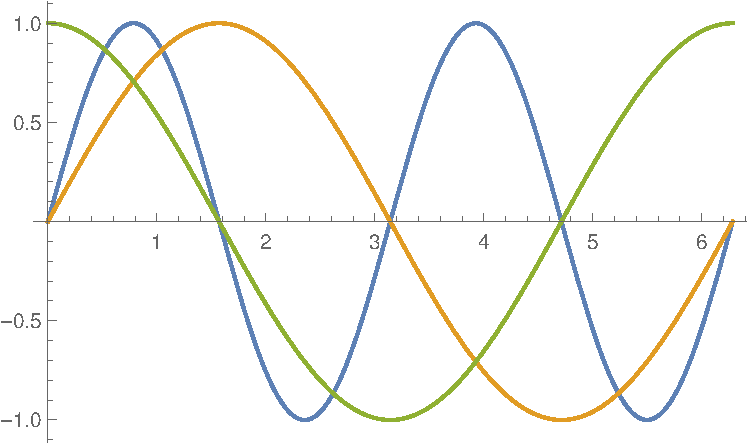
\includegraphics[scale=0.5]{f3.pdf}}
\end{center}
\end{frame}

\begin{frame}{van de Walls-en ekuazia (Gas Errealak)}

	\[ (P+\frac{n^2 a }{V^2})(V-nb)=nRT \]



	\[ a=7.857 \frac{L^2bar}{mol^{2}} \]
	\[ b=0.087 \frac{L}{mol} \]
	\[ R=0.0831 \frac{Lbar}{Kmol}\]

	\onslide<2->{ \[ P=\frac{RT}{Vm-b}-\frac{a}{Vm^2} \]}
\end{frame}

\begin{frame}{van de Walls-en ekuazia (Gas Errealak)}


	P[{\color{green}{\em Bm\_ }}, {\color{green}{\em T\_ }}] := R {\color{green}{\em T}} /({\color{green}{\em Bm}} -
	b) - a/{\color{green}{\em Bm}}$^2$ 

	\onslide<2->{Plot[P[{\color{blue}{Bm}}, 300], \{{\color{blue}{Bm}}, 0, 10\}, PlotRange -> \{\{0, 10\}, \{0, 40\}\}]}
	\vspace{1cm}
	\begin{center}
		\onslide<3->{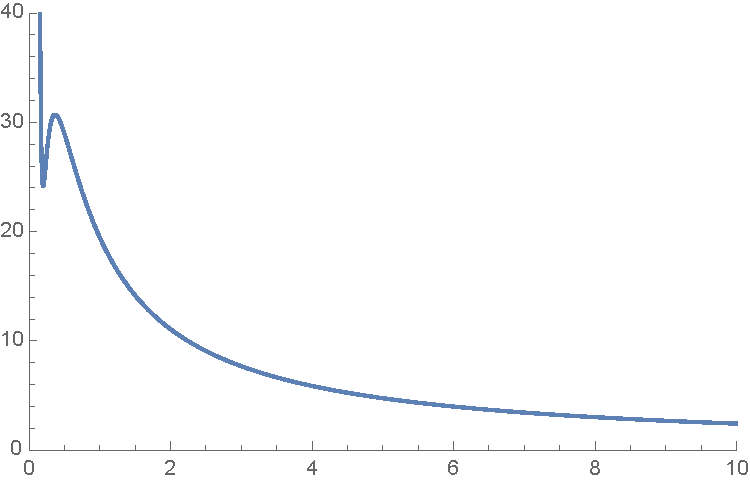
\includegraphics[scale=0.5]{f4.pdf}}
	\end{center}

\end{frame}
\begin{frame}{van de Walls-en ekuazia (Gas Errealak)}

	t300 = Plot[P[{\color{blue}{Bm}}, 300], \{ {\color{blue}{Bm}}, 0, 1\}, \\
	PlotRange -> \{\{0, 1\}, \{20, 70\}\}, Frame -> True, FrameLabel -> \{Style[Row[\{"Bolumen Murriztua ", Bm\}], 14], \\
Style[Row[\{"Presioa ", P\}], 14]\}, PlotLegends -> \{"300"\}];
\vspace{.8 cm}



t310 = Plot[P[{\color{blue}{Bm}}, 310], \{{\color{blue}{Bm}}, 0, 1\}, PlotStyle -> \{\{Thick, Green\}\},
PlotRange -> \{\{0, 1\}, \{20, 70\}\}, PlotLegends -> \{"310"\}];
\vspace{.8 cm}

Show[t300, t310]


\end{frame}
\begin{frame}{van de Walls-en ekuazia (Gas Errealak)}

	Manipulate[ Plot[P[{\color{blue}{Bm}}, {\color{blue}{T}}], \{ {\color{blue}{Bm}}, 0, 1\}, PlotRange -> \{\{0, 1\},
	\{20, 70\}\}, 
	PlotLegends -> \{{\color{blue}{T}} \}], \{{\color{blue}{T}}, 300, 380, 5\}]

\end{frame}

\section{ Partikula bat Kaxa batean }

\begin{frame}{Partikula bat Kaxa batean}
\[
V(x)=\left\{ \begin{array}{lll}
\infty & \textsf{ baldin eta }x<0 & \textsf{(I)}\\
0 & \textsf{ baldin eta }0\leq x\leq L & \textsf{(II)}\\
\infty & \textsf{ baldin eta }x>L & \textsf{(III)}
\end{array}\right.
\]
	
\begin{equation*}
	\Hat{H}(x)=-\dfrac{\hbar^{2}}{2m}\left(\dfrac{\partial^{2}}{\partial x^{2}}\right) + V(x)
%+\dfrac{\partial^{2}}{\partial y^{2}}+\dfrac{\partial^{2}}{\partial z^{2}}\right)=\Hat{h}_{x}+\Hat{h}_{y}+\Hat{h}_{z}.
\end{equation*}

\onslide<2->{ I eta III Zonak \ensuremath{V\to\infty\Rightarrow\psi_{I}(x)=\psi_{III}(x)=0}}

\end{frame}



\begin{frame}{Partikula bat Kaxa batean}
\begin{itemize}
\item II Zona 
	\begin{itemize}
		\item Jarraia, deribatu jarraia, integragarria ...
		\item Unibokoa -> $\psi(x=0)$ eta $\psi(x=L)$ 0 izan beharko da.
	\end{itemize}
\end{itemize}

\only<2>{\[ \psi^{\prime\prime}=-\dfrac{2m(E-V)}{\hbar^{2}}\psi \] }
\only<3->{\[ \psi^{\prime\prime}=-\dfrac{2mE}{\hbar^{2}}\psi \] }
\only<2>{non V=0.}

\vspace{-0.25 cm}
%{\tiny{}
\onslide<4->{\[
	\psi_{II}(x)=Asin{kx}+Bcos{kx}
\]}

\end{frame}


\begin{frame}{Partikula bat Kaxa batean}
Uhin-funtzioa jarraia izan dadin :
\begin{itemize}
\item<1->  $ \psi_{\mathsf{I}}(x=0)=\psi_{\mathsf{II}}(x=0)=0\quad\Rightarrow\quad B=0 $
\[
	\psi_{II}(x)=Asin{kx}  
\] 
\[ \psi^{\prime\prime}=-\dfrac{2mE}{\hbar^{2}}\psi \] 

{\tt \bf MATH. Zein da Energiaren expresioa?}
		\item<2-> $ \psi_{\mathsf{II}}(x=L)=\psi_{\mathsf{II}}(x=L)=0 $

{\tt \bf MATH. Zein da k-ren balioa?}

\end{itemize}
\end{frame}


\begin{frame}{Partikula bat Kaxa batean. Normalizazioa}
	\begin{itemize}
		\item $  \int^L_0 \psi(x)*\psi(x) dx =1 $
	\end{itemize}
	{\tt \bf MATH. }

\end{frame}

\begin{frame}{Partikula bat Kaxa batean. Energia.}

	\onslide<2->{	\[ E = \frac{h^2}{8m}\frac{n^2}{L^2} \]}
	\onslide<3->{	\[ E = \frac{h^2}{8m}\left(\frac{nx^2}{L^2_x}+\frac{ny^2}{L^2_y}+\frac{nz^2}{L^2_z}\right) \]}

\end{frame}
\begin{frame}{Partikula bat Kaxa batean. Grafikak.}

\end{frame}





\begin{frame}{Partikula bat Kaxa batean. 3D}
	
\begin{equation*}
\Hat{H}=\Hat{T}=-\dfrac{\hbar^{2}}{2m}\left(\dfrac{\partial^{2}}{\partial x^{2}}+\dfrac{\partial^{2}}{\partial y^{2}}+\dfrac{\partial^{2}}{\partial z^{2}}\right)=\Hat{h}_{x}+\Hat{h}_{y}+\Hat{h}_{z}.
\end{equation*}

\begin{center}
\onslide<2->{$ \psi(x,y,z)=\psi(x)\psi(y)\psi(z) $}\\
\vspace{0.7cm}
\onslide<3->{$ E_{Totala}=E(x)+E(y)+E(z) $}
\end{center}
%\[
%\Hat{H}=\Hat{T}=-\dfrac{\hbar^{2}}{2m}\left(\dfrac{\partial^{2}}{\partial x^{2}}+\dfrac{\partial^{2}}{\partial y^{2}}+\dfrac{\partial^{2}}{\partial z^{2}}\right)=\Hat{h}_{x}+\Hat{h}_{y}+\Hat{h}_{z}.
%
%\]
\end{frame}

\section{ Hidrogeno Atomoa }
\end{document}
